This manuscript
(\href{https://MMV-Lab.github.io/im2im-paper/v/af028ce9536fb8f3682322c0e67b0e9e211b5ff8/}{permalink})
was automatically generated
from \href{https://github.com/MMV-Lab/im2im-paper/tree/af028ce9536fb8f3682322c0e67b0e9e211b5ff8}{MMV-Lab/im2im-paper@af028ce}
on March 14, 2023.

\hypertarget{authors}{%
\subsection{Authors}\label{authors}}

\begin{itemize}
\item
  \textbf{Justin Sonneck}
  
\includegraphics[width=0.16667in,height=0.16667in]{images/orcid.svg}
  \href{https://orcid.org/0000-0002-1640-3045}{0000-0002-1640-3045}
  · 
\includegraphics[width=0.16667in,height=0.16667in]{images/github.svg}
  \href{https://github.com/Justin-Sonneck}{Justin-Sonneck}
  · 
\includegraphics[width=0.16667in,height=0.16667in]{images/twitter.svg}
  \href{https://twitter.com/JustinSonneck}{JustinSonneck}
  Leibniz-Institut für Analytische Wissenschaften - ISAS - e.V.
  · Funded by The Federal Ministry of Education and Research (BMBF) under the funding reference 161L0272
\item
  \textbf{Jianxu Chen}
  \textsuperscript{\protect\hyperlink{correspondence}{✉}}
  
\includegraphics[width=0.16667in,height=0.16667in]{images/orcid.svg}
  \href{https://orcid.org/0000-0002-8500-1357}{0000-0002-8500-1357}
  · 
\includegraphics[width=0.16667in,height=0.16667in]{images/github.svg}
  \href{https://github.com/jxchen01}{jxchen01}
  · 
\includegraphics[width=0.16667in,height=0.16667in]{images/twitter.svg}
  \href{https://twitter.com/JianxuChen}{JianxuChen}
  Leibniz-Institut für Analytische Wissenschaften - ISAS - e.V.
  · Funded by The Federal Ministry of Education and Research (BMBF) under the funding reference 161L0272
\end{itemize}

\hypertarget{abstract}{%
\subsection{Abstract}\label{abstract}}

The deep learning research in computer vision has been growing extremely fast in the past decade, many of which have been translated into novel image analysis methods for biomedical problems. Broadly speaking, many deep learning based biomedical image analysis methods can be considered as a general image-to-image transformation framework. In this work, we introduce a new open source python package \textbf{MMV\_Im2Im} for image-to-image transformation in bioimaging applications. The overall package is designed with a generic image-to-image transformation framework, which could be directly used for semantic segmentation, instance segmentation, image restoration, image generation, etc. The implementation takes advantage of the state-of-the-art machine learning engineering techniques for users to focus on the research without worrying about the engineering details. We demonstrate the effectiveness of \textbf{MMV\_Im2Im} in more than ten different biomedical problems. For biomedical machine learning researchers, we hope this new package could serve as the starting point for their specific problems to stimulate new biomedical image analysis or machine learning methods. For experimental biomedical researchers, we hope this work can provide a holistic view of the image-to-image transformation concept with diverse examples, so that deep learning based image-to-image transformation could be further integrated into the assay development process and permit new biomedical studies that can hardly be done only with traditional experimental methods. Source code can be found at \url{https://github.com/MMV-Lab/mmv_im2im}.

\hypertarget{introduction}{%
\subsection{Introduction}\label{introduction}}

With the rapid advancements in the fields of machine learning (ML) and computer vision, computers can now transform images into new forms, enabling better visualization {[}\protect\hyperlink{ref-1O0bopKD}{1}{]}, better animation {[}\protect\hyperlink{ref-LxlUp436}{2}{]} and better information extraction {[}\protect\hyperlink{ref-11chATuF4}{3}{]} with unprecedented and continuously growing accuracy and efficiency compared to conventional digital image processing.
These techniques have recently been adapted for bioimaging applications and have revolutionized image-based biomedical research {[}\protect\hyperlink{ref-Yq8wZ6hc}{4},\protect\hyperlink{ref-WwenuBHa}{5},\protect\hyperlink{ref-wcCVn8av}{6},\protect\hyperlink{ref-xPgDok51}{7}{]}. In principal, these techniques and applications can be formulated as a general image-to-image transformation problem, as depicted in the central panel in Figure \ref{fig:overview}. Deep neural networks are trained to perceive the information from the source image(s) and reconstruct the learned knowledge from source images(s) in the form of a new image(s) of the target type.
The source and target images can be real or simulated microscopy images, segmentation masks, or their combinations, as exemplified in Figure \ref{fig:overview}.
Since these underlying methods share the same essential spirit, a natural question arises: is it possible to develop a single generic codebase for deep learning-based image-to-image transformation applicable to various biomedical studies?

In this paper, we introduce \emph{MMV\_Im2Im} an open-source microscopy machine vision (MMV) toolbox for image-to-image transformation and demonstrate its applications in over 10 biomedical applications of various types.
Currently, \emph{MMV\_Im2Im} supports 2D\textasciitilde5D microscopy images for supervised image-to-image translation (e.g., labelfree determination {[}\protect\hyperlink{ref-Yq8wZ6hc}{4}{]}, imaging modality transformation {[}\protect\hyperlink{ref-WwenuBHa}{5},\protect\hyperlink{ref-UEBDZ3tI}{8}{]}), supervised image restoration {[}\protect\hyperlink{ref-wcCVn8av}{6}{]}, supervised semantic segmentation {[}\protect\hyperlink{ref-TutLhFSz}{9}{]}, supervised instance segmentation {[}\protect\hyperlink{ref-K2ugNcVa}{10},\protect\hyperlink{ref-QmYuUQ5K}{11}{]}, unsupervised semantic segmentation {[}\protect\hyperlink{ref-RuFP3CS3}{12}{]}, unsupervised image to image translation and synthetization {[}\protect\hyperlink{ref-6wtIu4QY}{13}{]}.
The toolbox will continuously grow with more and more methods especially methods based on self-supervised learning, ideally with community contributions.

Why do we need such a single generic codebase for all deep-learning based microscopy image-to-image transformation? \emph{MMV\_Im2Im} is not simply a collection of many existing methods, but with rather systematic design for generality, flexibility, simplicity and reusability, attempting to address many fundamental pain points for image-to-image transformation in biomedical applications, as highlighted below.

\hypertarget{feature-1-universal-boilerplate-with-state-of-the-art-ml-engineering}{%
\subsubsection{Feature 1: universal boilerplate with state-of-the-art ML engineering:}\label{feature-1-universal-boilerplate-with-state-of-the-art-ml-engineering}}

Targeted pain point: code from others may not be easy to understand or to extend or re-use. \emph{MMV\_Im2Im} employs pytorch-lightning {[}\protect\hyperlink{ref-YbvSvdyB}{14}{]} as the core in the backend, which offers numerous benefits, such as readability, flexibility, simplicity and reusability. First of all, have you ever had the moment when you wanted to extend the someone's open-source code to suit your special ML needs, but found it so difficult to figure out where and how to extend, especially for complex methods? Or, have you ever encountered the situation where you want to compare the methods and code from two different papers, even solving the same problem, e.g.~semantic segmentation, but not quite easy to grasp quickly since the two repositories are implemented in very different ways? It is not rare that even different researchers from the same group may implement similar methods in very different manners. This is not only a barrier for other people to learn and re-use the open-source code, but also poses challenges for developers in maintenance, further development, and interoperability among different packages.
We follow the pytorch-lightning framework and carefully design a universal boilerplate for image-to-image transformation for biomedical applications, where the implementation of all the methods share the same modularized code structure. This greatly lowers the learning curve for people to read and understand the code, and makes implementing new methods or extending existing methods simple and fast, at least from an engineering perspective.

Moreover, as ML scientists, have you ever overwhelmed by different training tricks for different methods or been curious about if certain state-of-the-art training methods can boost the performance of existing models? With the pytorch-lightning backend, \emph{MMV\_Im2Im} allows you to enjoy different state-of-the-art ML engineering techniques without changing the code, e.g., stochastic weight averaging {[}\protect\hyperlink{ref-qzeQFRn9}{15}{]}, single precision training, automatic batch size determination, different optimizers, different learning rate schedulers, easy deployment on different devices, distributed training on multi-GPU (even multi-node), logging with common loggers such as Tensorboard, etc.. In short, with the pytorch-lightning based universal boilerplate, bioimaging researchers can really focus on research and develop novel methods for their biomedical applications, without worrying about the ML engineering works (which are usually lack in non-computer-science labs).

\hypertarget{modularization-and-human-readable-configuration-system}{%
\subsubsection{Modularization and human-readable configuration system:}\label{modularization-and-human-readable-configuration-system}}

The toolbox is designed for both people with or without extensive experience with ML and Python programming.\\
For this purpose, we design the toolbox in a systematically modularized way with various levels of configurability.
One can use the toolbox with a single command as simple as \texttt{run\_im2im\ -\/-config\ train\_semanticseg\_3d\ -\/-data.data\_path\ /path/to/data} or make customization on details directly from a human-readable configuration file, such as choosing batch normalization or instance normalization in certain layers of the model, or adding extra data augmentation steps, etc.. For users without experience in Python programming, another graphical MMV toolbox has been planned as the extension of \emph{MMV\_Im2Im} (see Discussion for details).

In addition, the modularization and configuration system is designed to allow not only configuring with the elements offered by the package itself, but also any compatible elements from a third-party package or from a public repository on Github.
For example, one can easily switch the 3D neural network in the original \emph{Embedseg} method to any customized U-Net from FastAI by specifying the network as \texttt{fastai.vision.models.unet}. Such painless extendability releases the power of the toolbox, amplifies the benefit of the open-source ML community and upholds our philosophy of open science.

\hypertarget{customization-for-biomedical-imaging-applications}{%
\subsubsection{Customization for biomedical imaging applications:}\label{customization-for-biomedical-imaging-applications}}

The original idea of a general toolbox actually stememd from the OpenMMLab project (\url{https://openmmlab.com/}), which provides generic codebase for a wide range of computer vision research topics.
For instance, \emph{MMSegmentation} (\url{https://github.com/open-mmlab/mmsegmentation}) is an open source toolbox for semantic segmentation, supporting unified benchmarking and state-of-the-art models ready to use out-of-box.
It has become one of most widely used codebase for research in semantic segmentation (2K forks and 5.4K stars on Github as of March 12, 2023).
This inspires us to develop \emph{MMV\_Im2Im} to fascinate research in image-to-image transformation with special focus on biomedical applications.

First of all, different from general computer vision datasets, such as ImageNet {[}\protect\hyperlink{ref-lt4BNUoG}{16}{]}, where the images are usually small 2D RGB images (e.g., 3 x 256 x 256 pixels), biomedical applications usually involves large-scale high dimensional data (e.g., 4 x 128 x 2048 x 2048 voxels). To deal with this issue, we employ the PersistentDataset in MONAI {[}\protect\hyperlink{ref-UU62HYC6}{17}{]} with partial loading and sampling support, as well as delayed image reading in aicsimageio {[}\protect\hyperlink{ref-ONdyoUIo}{18}{]} as default (configuraable if other dataloaders are preferred).
As a result, in our stress test, training an 3D nuclei instance segmentation model with more than 125,000 3D images can be conducted efficiently, even with limited resource.

Second, because microscopy data is not restricted to 2D, we re-implement common frameworks, such as fully convolutional networks (FCN), conditional generative models, cycle-consistent generative models, etc., in a generic way to easily switch between different dimensionalities.

Third, the toolbox pre-packs common functionalities specific to microscopy images. For example, we incorporate the special image normalization method introduced in {[}\protect\hyperlink{ref-Yq8wZ6hc}{4}{]}, where only the middle chunk along Z dimension of 3D microscopy images will be used for calculating the mean and standard deviation of image intensity for standard normalization. Also, 3D light microscopy images are usually anisotropic, i.e., much lower resolution along Z than XY dimension. So, we adopt the anisotropic variation of UNet as proposed in {[}\protect\hyperlink{ref-jM3v1UjQ}{19}{]}.

Finally, to deploy the model in production, a model trained on small 3D patches sometimes need to be applied not only on much large images, but also with additional dimensionalities (e.g., multi-scene timelapse). Combining the efficient data handling of aicsimageio {[}\protect\hyperlink{ref-ONdyoUIo}{18}{]} and the sliding window inference with gaussian weighted blending, the toolbox can yield efficient inference without visible stitching artifacts in production.

All in all, the \emph{MMV\_Im2Im} toolbox stands on the shoulders of many giants in the open-source software and ML engineering communities (pytorch-lightning, MONAI, aicsimageio, etc.) and is systematically designed for image-to-image transformation R\&D for biomedical applications. The source code of \emph{MMV\_Im2Im} is available at \url{https://github.com/MMV-Lab/mmv_im2im}. This manuscript is generated with open-source package Manubot {[}\protect\hyperlink{ref-YuJbg3zO}{20}{]}. The manuscript source code is available at \url{https://github.com/MMV-Lab/im2im-paper}.

\begin{figure}
\hypertarget{fig:overview}{%
\centering
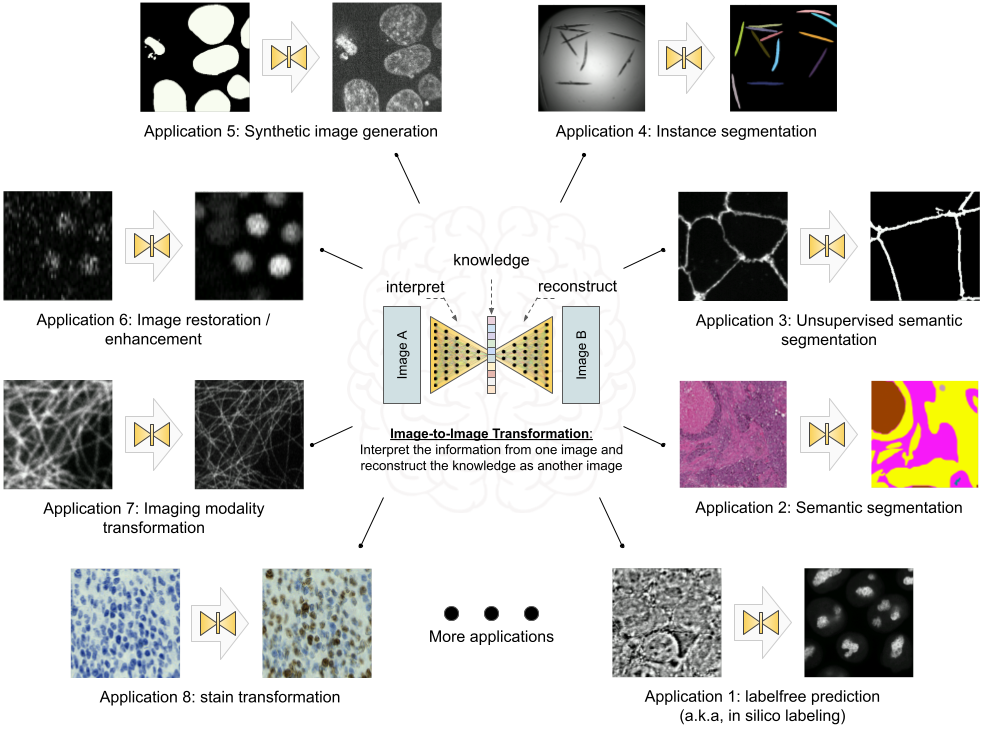
\includegraphics[width=1\textwidth,height=0.53\textheight]{images/overview_figure.png}
\caption{Overview of the image-to-image transformation concept and its example applications.}\label{fig:overview}
}
\end{figure}

\hypertarget{results}{%
\subsection{Results}\label{results}}

In this section, we showcase the versatility of the \emph{MMV\_Im2Im} toolbox by presenting over ten different biomedical applications across various R\&D use cases and scales. All experiments and results in this section were conducted on publicly available datasets and our scripts (for pulling the public dataset online and data wrangling) and configuration files (for setting up training and inference details), both included in the MMV\_Im2Im package, enable easy reproduction of the results. It is important to note that the aim of these experiments was not to achieve state-of-the-art performance on each individual task, as this may require further hyper-parameter tuning (see Discussion section for more details). Rather, the experiments were intended to demonstrate the package's different features and general applicability, providing a holistic view of image-to-image transformation concepts to biomedical researchers. We hope that these concepts will help researchers better integrate AI into traditional assay development strategies and inspire computational and experimental co-design methods, enabling new biomedical studies that were previously unfeasible.

\hypertarget{labelfree-prediction-of-nuclear-structure-from-2d3d-brightfield-images}{%
\subsubsection{Labelfree prediction of nuclear structure from 2D/3D brightfield images}\label{labelfree-prediction-of-nuclear-structure-from-2d3d-brightfield-images}}

The labelfree method refers a deep learning method that can predict fluorescent images directly from transmitted light brightfield images {[}\protect\hyperlink{ref-Yq8wZ6hc}{4}{]}. Comparing to brightfield images, fluorescent images can resolve subcellular structures in living cells at high resolution but with the cost of expensive and slow procedures and high phototoxicity. The labelfree method provides a new perspective in assay development to conduct integrated computational analysis of multiple organelles only with a single brightfield imaging acquisition. In our first demonstration, we applied \emph{MMV\_Im2Im} to build 2D/3D models that can predict fluorescent images of nuclear structures from brightfield images. For 3D models, we also compared (1) different image normalization methods, (2) different network backbones, and (3) different types of models.

It should be noted that while we recognize the importance of systematically evaluating our prediction, such an analysis falls outside the scope of this paper. We argue that the proper evaluation methodology should depend on specific downstream quantitative analysis goals (e.g., {[}\protect\hyperlink{ref-gPpwGUco}{21},\protect\hyperlink{ref-EOO2mf0p}{22}{]}). For example, if our aim is to quantify the size of nucleoli, we must compare the segmentation derived from real nucleoli signals to that of the predicted nucleoli segmentation, ensuring that measurements from both are consistent. Alternatively, if the goal is to localize the nucleoli roughly within the cell, Pearson correlation may be a more appropriate metric. In this work, we concentrate on visual inspection, using Pearson correlation and structural similarity as a rough quantitative reference. Our intent is to demonstrate the utility of our \emph{MMV\_Im2Im} package, and leave systematic evaluations to users in their specific problems in real studies.

\emph{2D Labelfree:} We started with a simple problem using 2D images from the HeLa ``Kyoto'' cells dataset {[}\protect\hyperlink{ref-xv2VIyRP}{23}{]}. For all images, we took the brightfield channel and the mCherry-H2B channel out of the multi-channel timelapse movies. 2D images were acquired at 20x with 0.8 N.A. and then downscaled by 4 (pixel size: 0.299 nm x 0.299 nm). Example predictions can be found in Figure \ref{fig:labelfree}-A. We compared a basic UNet model {[}\protect\hyperlink{ref-TutLhFSz}{9}{]} and a 2D version of the fnet model in {[}\protect\hyperlink{ref-Yq8wZ6hc}{4}{]}. The fnet model achieved slightly more accurate predictions than basic UNet.

\emph{3D Labelfree:} We tested with 3D images from the hiPS single cell image dataset {[}\protect\hyperlink{ref-5sGcmDuy}{24}{]}. Specifically, we extracted the brightfield channel and the structure channel from the full field-of-view (FOV) multi-channel images, from the HIST1H2BJ, FBL, NPM1, LMNB1 cell lines, so as to predict from one brightfield image various nuclear structures, histones, nucleoli (dense fibrillar component via fibrillarin), nucleoli (granular component via nucleophosmin), and nuclear envelope, respectively. Images were acquired at 100x with 1.25 NA. (voxel size: 0.108 micron x 0.108 micron x 0.29 micron).

We conducted three groups of comparisons (see results in Figure \ref{fig:labelfree})-B. First, we compared three different image normalization methods for 3D images: percentile normalization, standard normalization, center normalization {[}\protect\hyperlink{ref-Yq8wZ6hc}{4}{]}. Percentile normalization refers to cutting the intensity out of the range of {[}0.5, 99.5{]} percentile of the image intensity and then rescale the values to the range of {[}-1, 1{]}, while the standard normalization is simply subtracting mean intensity and then divided by the standard deviation of all pixel intensities. Center normalization is similar to standard normalization, but the statistics are calculated only around center along the Z-axis. One could easily test different percentile or rescaling to {[}0, 1{]} instead of {[}-1, 1{]}. Qualitatively, we found center normalization slightly more accurate and more robust than the other two (ref. the first row in Figure \ref{fig:labelfree}-B).

Second, we compared different network backbone architectures, including original fnet model {[}\protect\hyperlink{ref-Yq8wZ6hc}{4}{]}, enhanced UNet {[}\protect\hyperlink{ref-M7480NLD}{25}{]}, attention UNet {[}\protect\hyperlink{ref-OCow1hly}{26}{]}, two transformer-based models, SwinUNETR {[}\protect\hyperlink{ref-ZWL3IrVc}{27}{]} and UNETR{[}\protect\hyperlink{ref-XCKUntOB}{28}{]} (all with center normalization). Inspecting the predictions on a holdout validation set suggested that fnet achieved the best performance, and the recent transformer-based models did not work well with in labelfree problems (ref. the second row and the ``c + fnet'' from the first row in Figure \ref{fig:labelfree}-B).

Finally, we showed the comparison between three different types of models, an FCN-type model (i.e., fnet), a pix2pix-type model, and a cycleGAN-type model. For fair comparison, we used fnet as the same backbone for all three types of models. In theory, the pix2pix-type model can be trained in two different ways: from scratch or initializing the generator with a pre-trained fnet (trained as FCN). Examples of the comparison results were shown in the last two rows in Figure \ref{fig:labelfree}-B. Visually, it is evident that the additional adversarial components (i.e., the discriminator) could generate images with more realistic apprearnce than a typical FCN-type model alone, but again, we leave the systematic quantitative evaluations to users' specfic biomedical studies.

From the experiments above, we found that center normalization + pix2pix with fnet as the generator achieved the best overall performance. So, we employed the same strategy on all other nuclear structures. At the end, we had four different labelfree models, each predicting one different nuclear structure from 3D brightfield images. As an example of evaluation, we calculated the pearson correlation and structural similarity on the validation set. The results were summarized in Table \ref{tbl:labelfree_table}. Again, these numbers were merely examples of evaluation, systematic evaluation based each specific biological problem would be necessary before deployment. Figure \ref{fig:labelfree}-C showed one example of all four different structures predicted from a single unseen brightfield image. This would permit an integrated analysis of four different nuclear components that could hardly be acquired simultaneously in real experiments and real images.

\begin{longtable}[]{@{}
  >{\raggedright\arraybackslash}p{(\columnwidth - 6\tabcolsep) * \real{0.2500}}
  >{\raggedright\arraybackslash}p{(\columnwidth - 6\tabcolsep) * \real{0.2500}}
  >{\raggedright\arraybackslash}p{(\columnwidth - 6\tabcolsep) * \real{0.2500}}
  >{\raggedright\arraybackslash}p{(\columnwidth - 6\tabcolsep) * \real{0.2500}}@{}}
\caption{Evaluation of the final 3D label-free models for four different nuclear structures. \label{tbl:labelfree_table}}\label{tbl:labelfree_table}\tabularnewline
\toprule()
\begin{minipage}[b]{\linewidth}\raggedright
Dataset
\end{minipage} & \begin{minipage}[b]{\linewidth}\raggedright
Pearson Correlation
\end{minipage} & \begin{minipage}[b]{\linewidth}\raggedright
Structural Similarity
\end{minipage} & \begin{minipage}[b]{\linewidth}\raggedright
\# of Test Data
\end{minipage} \\
\midrule()
\endfirsthead
\toprule()
\begin{minipage}[b]{\linewidth}\raggedright
Dataset
\end{minipage} & \begin{minipage}[b]{\linewidth}\raggedright
Pearson Correlation
\end{minipage} & \begin{minipage}[b]{\linewidth}\raggedright
Structural Similarity
\end{minipage} & \begin{minipage}[b]{\linewidth}\raggedright
\# of Test Data
\end{minipage} \\
\midrule()
\endhead
FBL & 0.864 ± 0.021 & 0.831 ± 0.034 & 50 \\
HIST1H2BJ & 0.825 ± 0.034 & 0.675 ± 0.073 & 55 \\
LMNB1 & 0.853 ± 0.027 & 0.669 ± 0.059 & 50 \\
NPM1 & 0.912 ± 0.015 & 0.795 ± 0.039 & 55 \\
\bottomrule()
\end{longtable}

\begin{figure}
\hypertarget{fig:labelfree}{%
\centering
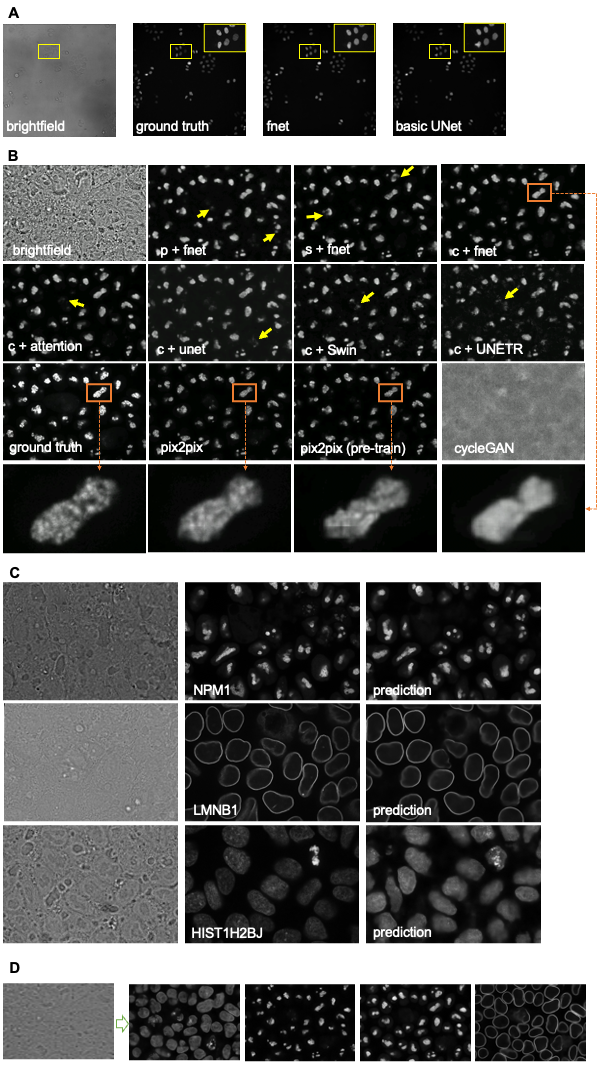
\includegraphics[width=0.76\textwidth,height=0.9\textheight]{images/labelfree.png}
\caption{Examples of labelfree results. p/c/s refers percentile normalization, center normalization, and standard normalization, respectively (see main text for details).}\label{fig:labelfree}
}
\end{figure}

\hypertarget{d-semantic-segmentation-of-tissues-from-he-images}{%
\subsubsection{2D semantic segmentation of tissues from H\&E images}\label{d-semantic-segmentation-of-tissues-from-he-images}}

Segmentation is a common image processing task, and can be considered as a special type of image-to-image transformation, where the generated images are segmentation masks. Deep learning based methods have achieved huge success in 2D semantic segmentation in biomedical images. In this example, we demonstrated \emph{MMV\_Im2Im} on a pathology application to segment glands from hematoxylin and eosin (H\&E) stained tissue images from the 2015 Gland Segmentation challenge {[}\protect\hyperlink{ref-45Sirz1X}{29},\protect\hyperlink{ref-XAffSYIR}{30}{]}. Stain normalization is an important pre-processing step in order to develop models robust to stain variation and tissue variations. \emph{MMV\_Im2Im} included a classic stain normalization method {[}\protect\hyperlink{ref-tQhnZyjK}{31}{]} as a pre-processing step. The effect of stain normalization can be observed in Figure \ref{fig:2d_gland}-A and B. We trained a simple attention UNet model {[}\protect\hyperlink{ref-OCow1hly}{26}{]}. Evaluated on the two different hold-out test sets, the model achieved F1-score, 0.883 and 0.888 on test set A and test set B, respectively. The performance was competitive comparing to the methods reported in the challenge report {[}\protect\hyperlink{ref-XAffSYIR}{30}{]}, especially with much more consistent performance across the two different test sets. Example results can be found in Figure \ref{fig:2d_gland}-C.

\begin{figure}
\hypertarget{fig:2d_gland}{%
\centering
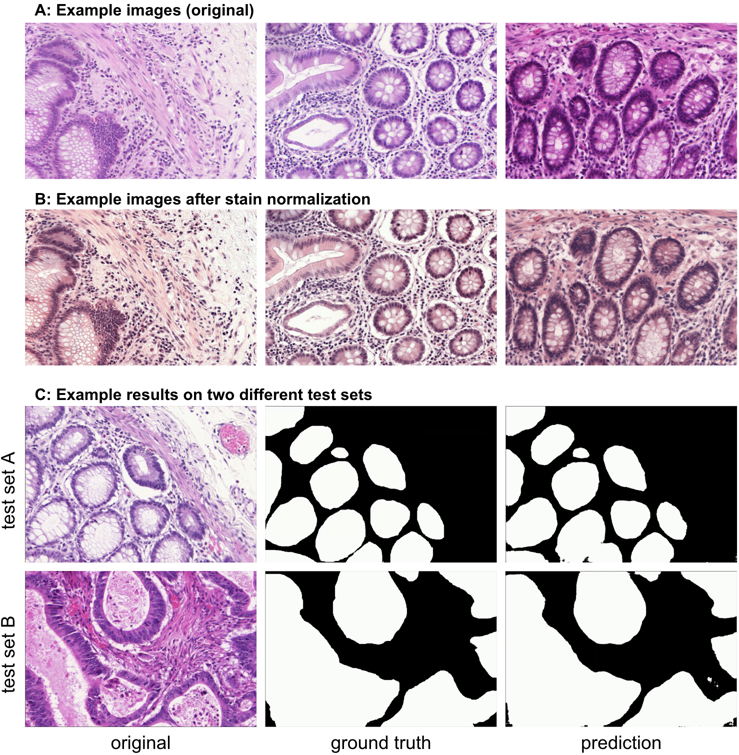
\includegraphics[width=0.75\textwidth,height=\textheight]{images/gland.png}
\caption{Example results of 2D semantic segmentation of gland in H\&E images.}\label{fig:2d_gland}
}
\end{figure}

\hypertarget{d-semantic-segmentation-of-organelles-from-electron-microscopy-images}{%
\subsubsection{3D semantic segmentation of organelles from electron microscopy images}\label{d-semantic-segmentation-of-organelles-from-electron-microscopy-images}}

Semantic segmentation in 3D biomedical image analysis application is not a simple generalization from 2D models by switching 2D operations with 3D operations, but with many practical challenges. Large GPU footprint is one of the biggest issues, which makes many training strategies common in 2D not feasible in 3D, e.g.~limited mini-batch size. \emph{MMV\_Im2Im} is able to take advantage of state-of-the-art ML engineering methods to efficiently handle 3D problems. For example, by using effective half-precision training, one can greatly reduce GPU memory workload for each sample and therefore increase the batch size. When multiple GPUs are available, it is also possible to easily take advantage of the additional resources to scale up the training to multiple GPU cards, even multiple GPU nodes. Here, we trained a 3D model to segment seven different types of organelles (e.g., cell, mitochondrion, alpha granule, etc.) from SBF-SEM image volumes {[}\protect\hyperlink{ref-3L5MIyIB}{32}{]}. Example results can be found in Figure \ref{fig:3dseg}. The prediction still suffered from considerable errors, very likely due to the limited training data (only one image).

\begin{figure}
\hypertarget{fig:3dseg}{%
\centering
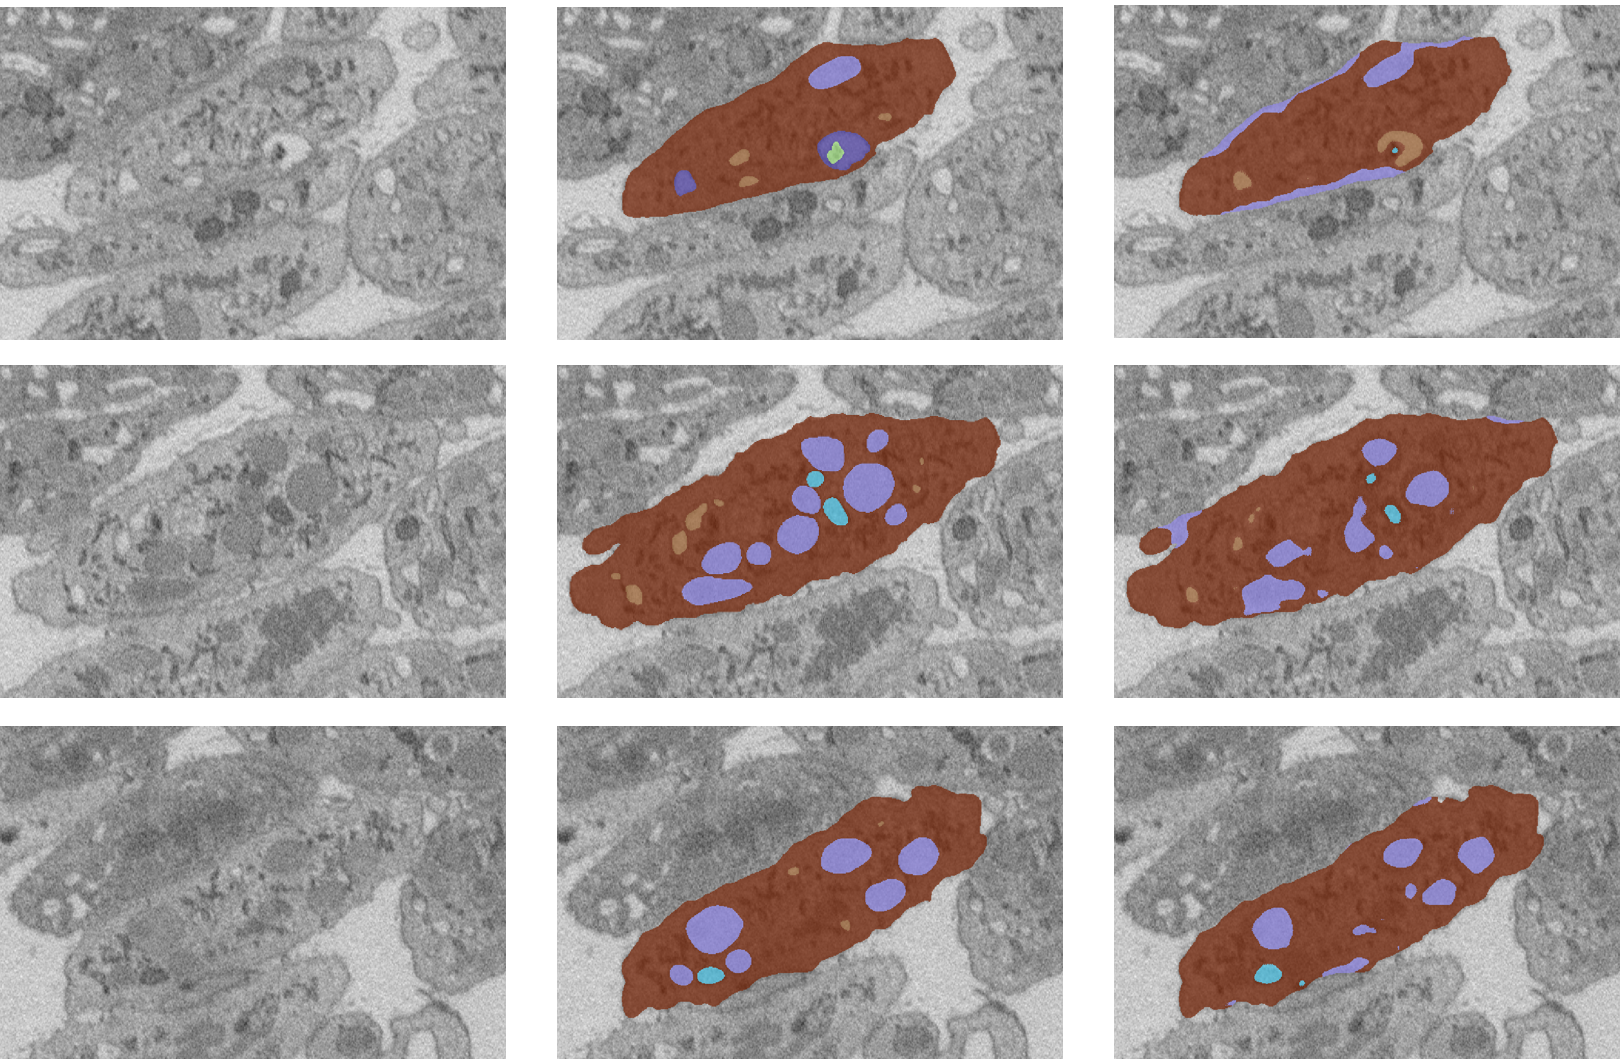
\includegraphics[width=0.75\textwidth,height=\textheight]{images/semantci_seg3d.png}
\caption{Result of 3D semantic segmentation results on z-slice 30, 60, 90. From left to right: raw images, ground truth, predictions.}\label{fig:3dseg}
}
\end{figure}

\hypertarget{unsupervised-semantic-segmentation-of-intracelluar-structures-from-2d3d-confocal-microscopy-images}{%
\subsubsection{Unsupervised semantic segmentation of intracelluar structures from 2D/3D confocal microscopy images}\label{unsupervised-semantic-segmentation-of-intracelluar-structures-from-2d3d-confocal-microscopy-images}}

Large amounts of high-quality segmentation ground truth is not always available, or may require endless effort to collect for a segmentation task. CycleGAN-based methods have opened up a new avenue for segmentation without the need for pixel-wise ground truth {[}\protect\hyperlink{ref-RuFP3CS3}{12}{]}. In this section, we demonstrate an unsupervised learning-based segmentation method on four examples: 2D tight-junction (via ZO1) segmentation from 2D FP-tagged ZO1 images (max-projected from 3D stacks), and segmentation of nuclei, mitochondria, and golgi from 3D confocal microscopy images.

To perform unsupervised learning, we used raw images from the hiPS single-cell image dataset {[}\protect\hyperlink{ref-5sGcmDuy}{24}{]}, as well as their corresponding segmentations (may not be absolute pixel-wise ground truth, but have gone through systematic evaluation to ensure the quality). We shuffled the raw images and their segmentations to generate a set of simulated segmentation masks, as suggested in {[}\protect\hyperlink{ref-RuFP3CS3}{12}{]}. While this approach may not be optimal, it serves as a simple demonstration of the concept, as illustrated in Figure \ref{fig:unsupervised}-A. Example results for all 3D models are shown in Figure \ref{fig:unsupervised}-B, and the F1-scores on the test set are summarized in Table \ref{tbl:unsuper}.

Interestingly, on the 2D ZO1 example, we observed that the segmentation generated by the unsupervised learning method was actually slightly better than the original segmentation obtained from a classic image segmentation workflow as in {[}\protect\hyperlink{ref-jM3v1UjQ}{19}{]}. For the 3D examples, it has been suggested {[}\protect\hyperlink{ref-RuFP3CS3}{12}{]} that the quality of unsupervised nuclei segmentation could be further improved with additional simulation strategies. Overall, we believe that unsupervised learning offers an effective way to generate preliminary segmentation, which can be further refined through active learning such as the iterative deep learning workflow described in {[}\protect\hyperlink{ref-jM3v1UjQ}{19}{]}

\begin{longtable}[]{@{}llll@{}}
\caption{F1 scores of the unsupervised semantic segmentation predictions. \label{tbl:unsuper}}\label{tbl:unsuper}\tabularnewline
\toprule()
Dimensionality & Dataset & F1 Score & \# of Test Data \\
\midrule()
\endfirsthead
\toprule()
Dimensionality & Dataset & F1 Score & \# of Test Data \\
\midrule()
\endhead
2D & tight-junction & 0.888 ± 0.022 & 29 \\
3D & nucleus & 0.811 ± 0.150 & 15 \\
3D & golgi & 0.705 ± 0.022 & 6 \\
3D & mitochondria & 0.783 ± 0.005 & 2 \\
\bottomrule()
\end{longtable}

\begin{figure}
\hypertarget{fig:unsupervised}{%
\centering
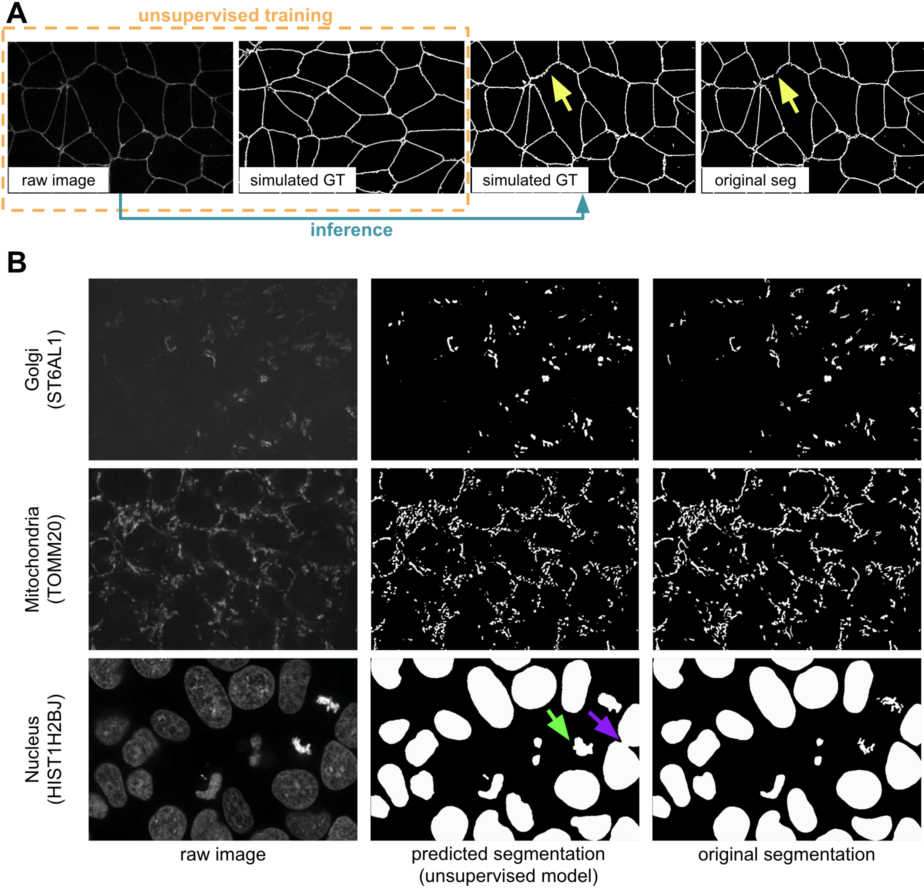
\includegraphics[width=0.9\textwidth,height=\textheight]{images/unsupervised.png}
\caption{(A) Illustration of the unsupervised learning scheme and results in the 2D tight-junction segmentation problem. The yellow arrows indicate a region where the unsupervised learning method actually predicted better than the original segmentation results by classic image processing methods. (B) Example 3D segmentation results (only showing a middle z-slice) from models obtained by unsupervised learning.}\label{fig:unsupervised}
}
\end{figure}

\hypertarget{instance-segmentation-in-microscopy-images}{%
\subsubsection{Instance segmentation in microscopy images}\label{instance-segmentation-in-microscopy-images}}

Instance segmentation is a type of segmentation problem that goes beyond semantic segmentation. The goal is to differentiate not only between different types of objects, but also different instances of the same type of objects. Currently, the \emph{MMV\_Im2Im} package supports \emph{EmbedSeg}-type models. The major benefit of EmbedSeg-type models is their agnosticism to the morphology and dimensionality of the objects, compared to other FCN-type models such as StarDist {[}\protect\hyperlink{ref-tIIG2f8K}{33},\protect\hyperlink{ref-14h90Vfg0}{34}{]} (which struggles with handling different shapes, such as elongated concave objects), and CellPose {[}\protect\hyperlink{ref-TugPkOLy}{35}{]} or SplineDist {[}\protect\hyperlink{ref-17Yrl6WGQ}{36}{]} (which are not straightforward to generalize to higher dimensions). For example, different from the others, \emph{EmbedSeg}-type models are even able to generate instance segmentation where each instance contains multiple connected components. Another mainstream category of instance segmentation methods are detection-based models, such as Mask-RCNN {[}\protect\hyperlink{ref-xi8wnibR}{37}{]}. However, these models are better suited to the detection framework rather than image-to-image transformation (see Discussion section for details).

The \emph{EmbedSeg}-type models were re-implemented according to the original paper {[}\protect\hyperlink{ref-K2ugNcVa}{10},\protect\hyperlink{ref-QmYuUQ5K}{11}{]} following the generic boilerplate in \emph{MMV\_Im2Im}, with significant improvment. First of all, following the modular design of \emph{MMV\_Im2Im}, it is flexible to use different neural network models as the backbone for \emph{EmbedSeg}. For 3D anisotropic microscopy image, the original backbone ERFNet {[}\protect\hyperlink{ref-XAkgs3Nh}{38}{]} doesn't take the anisotropic dimensions into account and therefore may not perform well or even not applicable. In this scenario, it is straighforward to employ another anisotropic neural network bone, such as the anisotropic U-Net in {[}\protect\hyperlink{ref-jM3v1UjQ}{19}{]} or the anisotropic version of Dynamic U-Net in MONAI. Second, we significantly improve training strategy. The original version requires pre-cropping patches and pre-calculated object centers around each individual instance. This may generate a massive amount of patches on the disk. More importantly, such pre-cropping makes data augmentation nearly impossible, except the simple ones like flipping (otherwise, the pre-calculated centers might be wrong), and also greatly undersamples around negative cases (e.g., background). For example, we have observed that for an Embedseg model training only with patches centered around an instance, the model may suffer from degraded performance during inference when there are a large amound of background pixels without any instances. Again, following the modular design of \emph{MMV\_Im2Im}, it is now possible to do on-the-fly data augmentation and patch sampling, even weighted patch sampling. Finally, our improved \emph{Embedseg}-type models can accept an exclusion mask so that certain parts of the images can be ignored during training. This is especially useful for partially annotated ground truth. For large images, it could be extremely time-consuming to require every single instance have to be annotated. The exclusion mask can effectively avoid this bottleneck. Another extension comparing to the original implementation was that the \emph{MMV\_Im2Im} package made sliding windowing inference straightforward, and therefore permitted easy handling of images of any size during inference in practice. As a demonstration, we applied \emph{EmbedSeg}-like models to a 2D problem of segmenting \emph{C. elegans} from widefield images {[}\protect\hyperlink{ref-138foKNOh}{39}{]}, as well as a 3D problem of nuclear segmentation from fluorescent and brightfield images from the hiPS single-cell image dataset {[}\protect\hyperlink{ref-5sGcmDuy}{24}{]}.

For the 2D problem, we adopted the same network backbone as in the original \emph{EmbedSeg} paper.
Example results on a small holdout set are shown in Figure \ref{fig:instance}-A (IoU = 0.86), which is comparable to the original published results {[}\protect\hyperlink{ref-QmYuUQ5K}{11}{]}.
For the 3D problem, the original backbone is not directly applicable, due to the aforementioned anisotropic issue and the images in the dataset do not contain enough Z-slices to run through all down sampling blocks in 3D. The segmentation results obtained from the public dataset {[}\protect\hyperlink{ref-5sGcmDuy}{24}{]} contain nuclear instance segmentation of all cells. But, the cells touch the image borders are ignored from downstream analysis and therefore not curated. In other words, the segmentation from this public dataset can only be used as high-quality nuclear instance segmentation ground truth after excluding the areas covered by cells touching the image borders {[}\protect\hyperlink{ref-5sGcmDuy}{24}{]}. Therefore, the exclusion masking function in \emph{MMV\_Im2Im} is very helpful in this example.

Example results were presented in \ref{fig:instance}-B. The green box highlighted a mitotic cell (the DNA signals forming ``spaghetti'' shapes). Besides roughly separating the DNA signals from background, the model was also able to correctly identify the instance identity, which would be theoretically infeasible for other FCN-type instance segmentation models.
Nuclear instance segmentation from brightfield images was much more challenging than from fluorescent images. Arguably, this could be thought of as one single model doing two transformations: predicting the DNA signals from brightfield and running instance segmentation on predicted DNA signals. From Figure \ref{fig:instance}-B, it was shown that the segmentation from brightfield images was comparable to the segmentation from fluorescent images, but with two caveats. First, the performance on mitotic cells was worse than the model using fluorescent images. We hypothesized this could be due to the limited information in brightfield images for mitotic cells, compounded with limited number of mitotic cells in the whole training set (less than 10\%). Second, the performance along Z dimension was also worse than the fluorescent model, as explained by the side view in Figure \ref{fig:instance}-B. This could be explained by the different properties of brightfield imaging and fluorescent imaging, but would need further comprehensive studies to investigate.

\begin{figure}
\hypertarget{fig:instance}{%
\centering
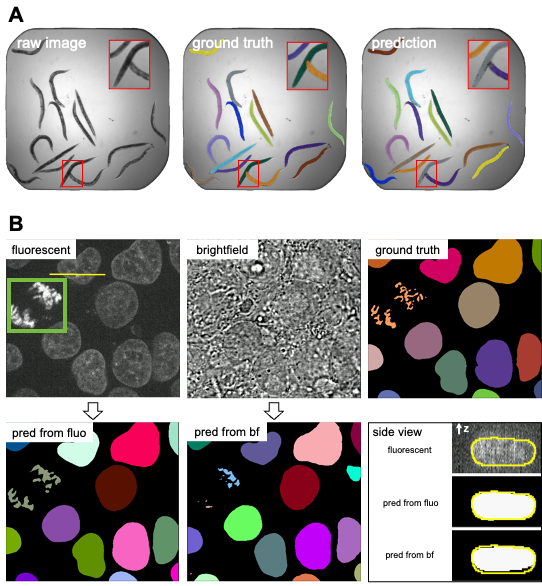
\includegraphics[width=0.85\textwidth,height=\textheight]{images/embedseg.png}
\caption{(A) Results 2D instance segmentation of C. elegans. Some minor errors can be observed in the zoom-in window, which could be refined with post-processing. (B) Results of 3D nuclear instance segmentation from fluorescent images and brightfield images. The green box in the fluorescent image highlights a mitotic example. The side view panel shows the segmentation of one specific nucleus along the line annotated in the fluorescent image from the side.}\label{fig:instance}
}
\end{figure}

\hypertarget{generating-synthetic-microscopy-images-from-binary-masks}{%
\subsubsection{Generating synthetic microscopy images from binary Masks}\label{generating-synthetic-microscopy-images-from-binary-masks}}

Generating a large amount of synthetic microscopy images can be an important step in developing image analysis methods. Synthetic images offer a way to train other deep learning models, such as self-supervised pre-training, using a diverse set of images without the need for large amounts of real-world data. As long as the synthetic images are generated with sufficient quality, it is possible to have an unlimited amount of training data for certain applications. Moreover, synthetic images can be used to evaluate other models when validation data is difficult to obtain. In this study, we demonstrate that \emph{MMV\_Im2Im} can generate 2D/3D synthetic microscopy images with high realism and validity, using a subset of data collected from the hiPS single-cell image dataset {[}\protect\hyperlink{ref-5sGcmDuy}{24}{]}, either in a supervised or unsupervised manner.

For a 3D demonstration, we conducted three different experiments, generating the nuclear segmentation from the dataset as input, and the real H2B images as the training target.

In the 2D case, we extracted the middle Z-slice from NPM1 images as the training target, while using the NPM1 segmentation results as the input binary mask. With the paired ``mask + microscopy image'' data, we could train the model in a supervised fashion, or randomly shuffle the data to simulate the situation without paired data and train the model in an unsupervised fashion. Example results can be found in Figure \ref{fig:synthetic}.

\begin{figure}
\hypertarget{fig:synthetic}{%
\centering
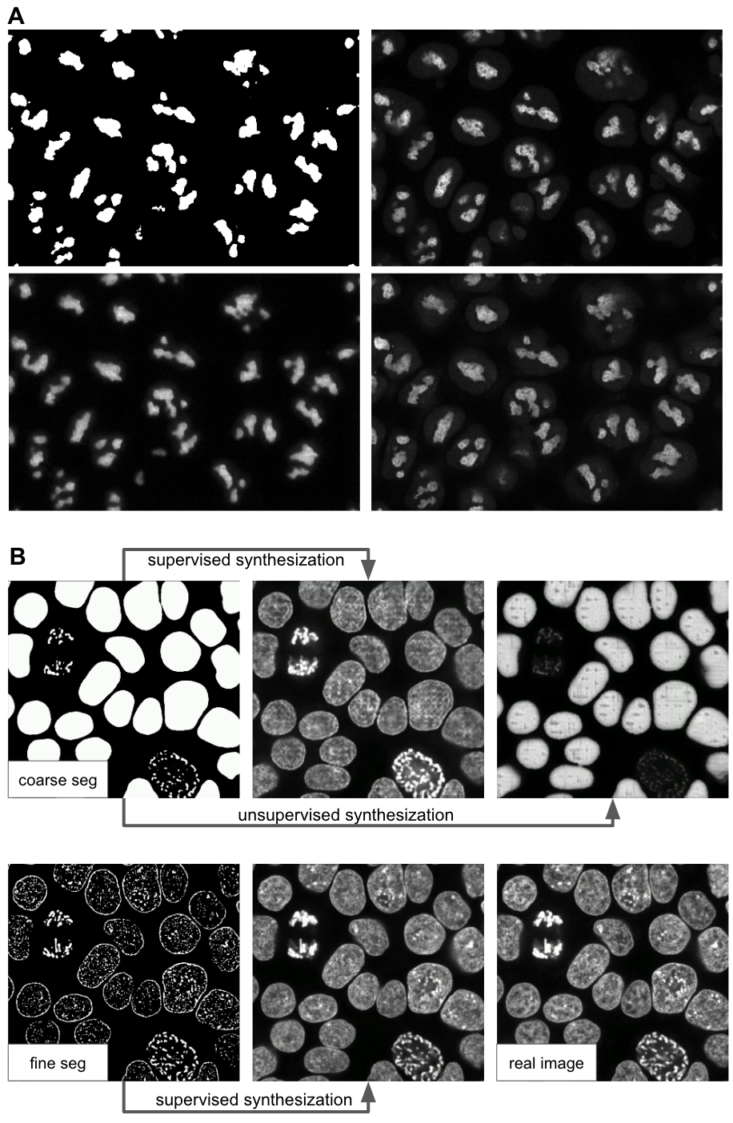
\includegraphics[width=0.6\textwidth,height=\textheight]{images/synthetic.png}
\caption{Example results of (A) 2D synthetic fluorescent images of NPM1 and (B) 3D synthetic fluorescent images of H2B (middle z-slices of two example z-stacks).}\label{fig:synthetic}
}
\end{figure}

\hypertarget{image-denoising-for-microscopy-images}{%
\subsubsection{Image denoising for microscopy images}\label{image-denoising-for-microscopy-images}}

\emph{MMV\_Im2Im} can also be used to computationally reduce image noise or restore the data from various sources of imaging artifacts, so as to increase the feasibility and efficiency in downstream analysis. In the current version of \emph{MMV\_Im2Im}, the restoration model can only be trained in a fully supervised manner. Therefore, aligned low quality and high quality images are required for supervision, even though such pair data can be partially simulated {[}\protect\hyperlink{ref-wcCVn8av}{6}{]}. Other methods, such as unsupervised learning based solutions {[}\protect\hyperlink{ref-4vnyY9J9}{41}{]}, will be made available within \emph{MMV\_Im2Im} in future versions.

In this example, we presented an image denoising demonstration with sample data from {[}\protect\hyperlink{ref-12G712Zky}{42}{]}. The goal was to increase the quality of low signal-to-noise ratio (SNR) images of nucleus-stained flatworm (Schmidtea mediterranea) and lightsheet images of Tribolium castaneum (red flour beetle) embryos. The models were trained with paired data acquired with low and high laser intensity on fixed samples, and then applied on live imaging data. For the nucleus-stained flatworm data (a test set of 20 images are available), the model achieved pearson correlation of 0.923 ± 0.029 and structural similarity of 0.627 ± 0.175. Based on the results in Figure \ref{fig:denoising}, it can be observed that the low SNR images can be greatly improved. Systematic quantitative evaluations would be necessary to confirm the biological validity, but beyond the scope of this paper.

\begin{figure}
\hypertarget{fig:denoising}{%
\centering
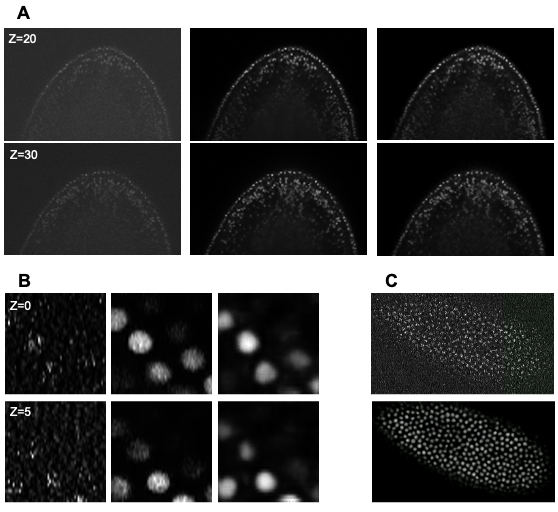
\includegraphics[width=0.75\textwidth,height=\textheight]{images/denoising.png}
\caption{(A) Denoising results of 3D images of nucleus-stained flatworm at two different z-slices. Left: raw images (low SNR), middle: reference images (high SNR), right: predictions. (B) Denoising results of 3D lightsheet images of Tribolium castaneum (fixed samples) at two different z-slices. Left: raw images (low SNR), middle: Reference images (high SNR), right: predictions. (C) Denoising results of 3D lightsheet images of Tribolium castaneum (live samples) without high SNR reference. Top: the raw image, bottom: the prediction.}\label{fig:denoising}
}
\end{figure}

\hypertarget{imaging-modality-transformation-from-3d-confocal-microscopy-images-to-stimulated-emission-depletion-sted-microscopy-images}{%
\subsubsection{Imaging modality transformation from 3D confocal microscopy images to stimulated emission depletion (STED) microscopy images}\label{imaging-modality-transformation-from-3d-confocal-microscopy-images-to-stimulated-emission-depletion-sted-microscopy-images}}

Another important application of image-to-image transformation is imaging modality transformation {[}\protect\hyperlink{ref-UEBDZ3tI}{8}{]}, usually from one ``cheaper'' modality with lower resolution (e.g., with larger field-of-view, easier to acquire and scale up) to another modality with higher resolution but expensive to obtain. Such models will permit a completely new way in assay development strategy to take advantage of all the benefits of the cheaper modality with lower resolution and still able to enhance the resolution computationally post hoc. To demonstrate the application of \emph{MMV\_Im2Im} in this scenario, we took an example dataset with paired 3D confocal and Stimulated Emission Depletion (STED) images of two different cellular structures, microtubule and nuclear pore {[}\protect\hyperlink{ref-UEBDZ3tI}{8}{]}. Sample results were summarized in Figure \ref{fig:modality}. For microtubule, the model achieved pearson correlation of 0.779 ± 0.019, while for nuclear pore complex, the pearson correlation was 0.784 ± 0.028. Also, visual inspection can confirm the effectiveness of the models. Again, it would be necessary to conduct further quantitative evaluation to ensure the validity in users' specific problems.

\begin{figure}
\hypertarget{fig:modality}{%
\centering
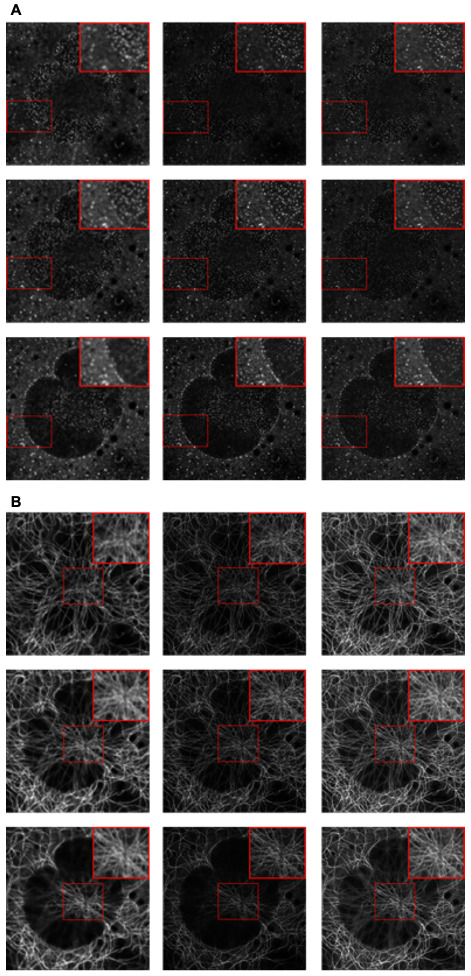
\includegraphics[width=0.65\textwidth,height=0.7\textheight]{images/modality.png}
\caption{Example results of confocal-to-STED modality transformation of nuclear pore (A) and microtubule (B) in three consecutive z-slices. From left to right: raw confocal images, reference STED images, predicted images.}\label{fig:modality}
}
\end{figure}

\hypertarget{staining-transformation-in-multiplex-experiments}{%
\subsubsection{Staining transformation in multiplex experiments}\label{staining-transformation-in-multiplex-experiments}}

Deep learning has emerged as a powerful tool for multiplex imaging, a powerful technique that enables the simultaneous detection and visualization of multiple biomolecules within a single tissue sample. This technique is increasingly being used in biomedical expereiements but demands efficient image analysis solutions to accurately identify and quantify the different biomolecules of interest at scale. Deep learning has demonstrated great potentials in analyzing muliplex datasets, as it can automatically learn the complex relationships between different biomolecules and their spatial distribution within tissues. Specially, in this study, we present the effectiveness of \emph{MMV\_Im2Im} in transforming tissue images from one staining to another, which will permit efficient co-registration, co-localization, and quantitative analysis of multiplex datasets. We used the sample dataset from {[}\protect\hyperlink{ref-WwenuBHa}{5}{]}. In this example, we trained three different models to transform IHC images to images of standard hematoxylin stain, mpIF nuclear (DAPI) and mpIF LAP2beta (a nuclear envelope stain). Example results can be observed in Figure \ref{fig:multiplex} to verify the results qualitatively. These transformed images can provide valuable insights into the localization and expression patterns of specific biomolecules spatially.

\begin{figure}
\hypertarget{fig:multiplex}{%
\centering
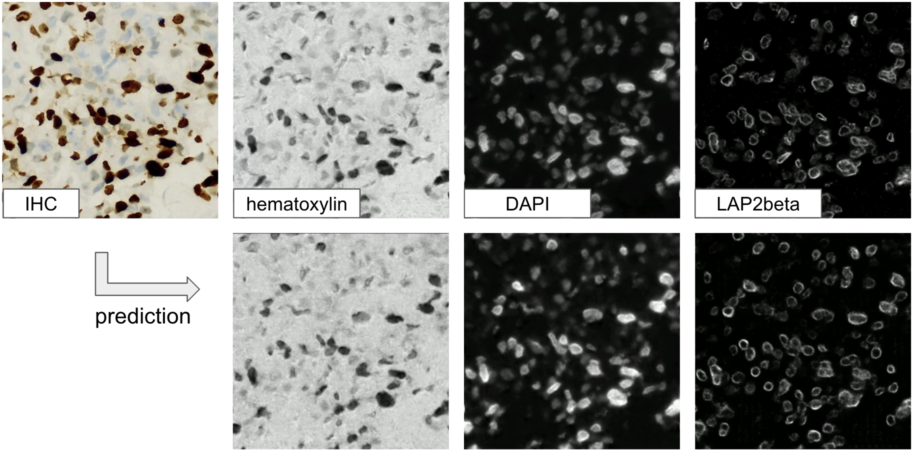
\includegraphics{images/multiplex.png}
\caption{Qualitative visualization of staining transformation results with the \emph{MMV\_Im2Im} package.}\label{fig:multiplex}
}
\end{figure}

\hypertarget{methods}{%
\subsection{Methods}\label{methods}}

\hypertarget{overview-of-the-code-base}{%
\subsubsection{Overview of the code base}\label{overview-of-the-code-base}}

Overall, the package inherited the boilerplate concept from pytorch-lightning (\url{https://www.pytorchlightning.ai/}), and was made fully configurable via yaml files supported by pyrallis (\url{https://github.com/eladrich/pyrallis}), as well as largely employed state-of-the-art deep learning components from MONAI (\url{https://monai.io/}). The three key parts in the package: mmv\_im2im.models, mmv\_im2im.data\_modules, and Trainers, will be further described below.

\hypertarget{main-frameworks-for-mmv_im2im.models}{%
\subsubsection{Main frameworks for mmv\_im2im.models}\label{main-frameworks-for-mmv_im2im.models}}

\emph{mmv\_im2im.models} is the core module defining the deep learning framework for your problem, where we can instantiate the neural network architecture and define what to do before training starts, what to do in each training and validation step, what to do at the end of each epoch, etc.. All implemented following the same lightning module from pytorch-lightning, which makes the code very easy to read, to understand, and even to extend.

In general, there are mainly four major deep learning frameworks that could be applied to microscopy image-to-image transformation: supervised learning with a fully convolutional networks (FCN) type models, supervised learning with pix2pix type models, unsupervised learning to learn mapping between visual domains, and Self2Self-type self-supervised learning {[}\protect\hyperlink{ref-srrRoFXR}{43}{]}. The major difference between FCN based supervised learning and pix2pix based supervised learning is that the pix2pix framework extends an FCN model with an adversarial head as a discriminator to further improves the realism of the prediction. The major difference between the unsupervised framework and the self-supervised framework is that the unsupervised methods still requires examples of the target images, even though the source images and target images do not need to be from the same sample or pixel-wise aligned. But, the self-supervised framework would only need the original images, which could be really helpful when it is impossible to acquire the target images (e.g., there is no truely noise-free or artifact-free image).

Currently, both the FCN-type and pix2pix-type supervised frameworks are well supported in the \emph{MMV\_Im2Im} package. Since our package is designed in a very generic way, it is possible to continuously expand the functionalities when available (ideally with community contributions). For example, diffusion models {[}\protect\hyperlink{ref-1A3yurr7m}{44}{]} can be thought of a modern extension of the pix2pix-type framework and therefore are within our horizon to include into \emph{MMV\_Im2Im}. For the unsupervised framework, only CycleGAN-type methods are supported. We are planning to extend the unsupervised framework with Imaginaire (\url{https://github.com/NVlabs/imaginaire}), which will greatly extend the applicability of \emph{MMV\_Im2Im} (e.g., learning the transformation from one single image to another single image or one set of images to another set of images). Meanwhile, supporting the self-supervised framework will be our next major milestone.

\hypertarget{customized-mmv_im2im.data_modules-for-bioimaging-applications}{%
\subsubsection{Customized mmv\_im2im.data\_modules for bioimaging applications}\label{customized-mmv_im2im.data_modules-for-bioimaging-applications}}

The \emph{data\_modules} implements a general module for data handling, from how to load the data to how to set up the dataloader for training and validation. Different people may prefer to organize their training data in different ways, such as using csv to organize input and the corresponding ground truth, or making different folders (e.g.~``image'' and ``ground\_truth'') with input and the corresponding ground truth sharing the same file name, etc.. Or some people may prefer to do a random train/validation split, while others like to pre-split train and validation into different folders, etc.. Currently, the \emph{data\_module} in \emph{MMV\_Im2Im} supports four different ways of data loading, where we try to cover as many common scenario as possible, so that everyone will feel comfortable using it.

A big challenge in the dataloader in bioimaging applications is that there could be not only a large amount of files, but also files of very large sizes. To deal with each individual large image, we used the delayed loading from aicsimageio for efficient image reading. Besides, we adopted the PersistentDataloader from MONAI to further optimize the efficiency. In specific, after loading a large image and running through all the deterministic operations, like intensity normalization or spatial padding, the PersistentDataLoader will pickle and save the data in a temporary folder, to avoid repeating the heavy computation on large files in each training iteration. To handle the potentially large number of files, we implemented the data\_module with capability of loading only a certain portion of the data into the memory in each epoch and reloading with a different portion every certain number of epochs. By doing this, we were able to efficiently train an instance segmentation model with more than 125K images, where each raw image is about 15MB.

\hypertarget{state-of-the-art-training-with-the-pytorch-lightning-trainer}{%
\subsubsection{State-of-the-art training with the pytorch-lightning Trainer}\label{state-of-the-art-training-with-the-pytorch-lightning-trainer}}

We fully adopted the Trainer from pytorch-lightning, which has been widely used by the machine learning community, and wildly tested on both R\&D problems and industrial-scale applications. In a nutshell, simply by specifying the training parameters in the yaml file, users can setup multi-GPU training, half-precision training, automatic learning rate finder, automatic batch size finder, early stopping, stochastic weight averaging, etc.. This allows users to focus on the research problems without worrying about the ML engineering.

\hypertarget{discussions}{%
\subsection{Discussions}\label{discussions}}

In this work, we presented a new open source python package \emph{MMV\_Im2Im} package for image-to-image transformations in bioimaging applications. We demonstrated the applicability on more than ten different problems or datasets to give biomedical researchers a holistic view of the general image-to-image transformation concepts with diverse examples. This package was not a simple collection of existing methods. Instead, we distilled the knowledge from existing methods and created this generic version with state-of-the-art ML engineering techniques, which made the package easy to understand, easy to use, and easy to extend for future. We hope this package can serve the starting point for other researchers doing AI-based image-to-image transformation research, and eventually build a large shared community in the field of image-to-image transformation for bioimaging.

One of main directions for extending \emph{MMV\_Im2Im} is to pre-pack common bioimaging datasets as a \emph{Dataset} module, so that users can easily test and benchmarking their method development. Besides the continuous improvement on the functionalities of the package, we also plan to develop two auxillary packages \emph{MMV\_Im2Im\_Auto} and \emph{MMV\_Im2Im\_Active}. In specific, when you have a reasonable amount of training data, MMV\_Im2Im\_Auto will take advantage of fact that \emph{MMV\_Im2Im} is fully configurable with yaml files, and automatically generate a set of potentially good configurations, then find the optimal solution for you. On the other hand, when you only have very limited training data, or even with only pseudo ground truth, \emph{MMV\_Im2Im\_Active} will help to build preliminary models from the limited training data, and gradually refine the model with human-in-the-loop by active learning. All the packages will also be wrapped into Napari plugins {[}\protect\hyperlink{ref-YEMgt2T4}{45}{]} to allow no-code operation and therefore be more friendly to users without experience in programming.

Finally, beyond \emph{MMV\_Im2Im}, we hope to build develop similar package for other problems (without re-inventing wheels). For example, as we mentioned in the instance segmentation application, Mask-RCNN type models are also very powerful instance segmentation methods and, in theory, can also be generalized beyond 2D images. However, Mask-RCNN would fit more to a detection framework, instead of image-to-image transformation. It will be supported in our \emph{MMV\_NDet} (NDet = N-dimensional detection) package.

\hypertarget{acknowledgments}{%
\subsection{Acknowledgments}\label{acknowledgments}}

We would like to thank the MONAI team for their support in our process of development, and the aicsimageio team for advices on how to integrate aicsimageio into the package. This work is supported by the Federal Ministry of Education and Research (Bundesministerium für Bildung und Forschung, BMBF) under the funding reference 161L0272.

\hypertarget{references}{%
\subsection{References}\label{references}}

\hypertarget{refs}{}
\begin{CSLReferences}{0}{0}
\leavevmode\vadjust pre{\hypertarget{ref-1O0bopKD}{}}%
\CSLLeftMargin{1. }%
\CSLRightInline{\textbf{Enhanced Deep Residual Networks for Single Image Super-Resolution}
\CSLBlock{Bee Lim, Sanghyun Son, Heewon Kim, Seungjun Nah, Kyoung Mu Lee} \emph{2017 IEEE Conference on Computer Vision and Pattern Recognition Workshops (CVPRW)} (2017-07) \url{https://doi.org/gfxhp3}
\CSLBlock{DOI: \href{https://doi.org/10.1109/cvprw.2017.151}{10.1109/cvprw.2017.151}}}

\leavevmode\vadjust pre{\hypertarget{ref-LxlUp436}{}}%
\CSLLeftMargin{2. }%
\CSLRightInline{\textbf{Image-to-Image Translation with Conditional Adversarial Networks}
\CSLBlock{Phillip Isola, Jun-Yan Zhu, Tinghui Zhou, Alexei A Efros} \emph{2017 IEEE Conference on Computer Vision and Pattern Recognition (CVPR)} (2017-07) \url{https://doi.org/gfrfv9}
\CSLBlock{DOI: \href{https://doi.org/10.1109/cvpr.2017.632}{10.1109/cvpr.2017.632}}}

\leavevmode\vadjust pre{\hypertarget{ref-11chATuF4}{}}%
\CSLLeftMargin{3. }%
\CSLRightInline{\textbf{Panoptic Segmentation}
\CSLBlock{Alexander Kirillov, Kaiming He, Ross Girshick, Carsten Rother, Piotr Dollar} \emph{2019 IEEE/CVF Conference on Computer Vision and Pattern Recognition (CVPR)} (2019-06) \url{https://doi.org/ggp9z4}
\CSLBlock{DOI: \href{https://doi.org/10.1109/cvpr.2019.00963}{10.1109/cvpr.2019.00963}}}

\leavevmode\vadjust pre{\hypertarget{ref-Yq8wZ6hc}{}}%
\CSLLeftMargin{4. }%
\CSLRightInline{\textbf{Label-free prediction of three-dimensional fluorescence images from transmitted-light microscopy}
\CSLBlock{Chawin Ounkomol, Sharmishtaa Seshamani, Mary M Maleckar, Forrest Collman, Gregory R Johnson} \emph{Nature Methods} (2018-09-17) \url{https://doi.org/gd7d5f}
\CSLBlock{DOI: \href{https://doi.org/10.1038/s41592-018-0111-2}{10.1038/s41592-018-0111-2} · PMID: \href{https://www.ncbi.nlm.nih.gov/pubmed/30224672}{30224672} · PMCID: \href{https://www.ncbi.nlm.nih.gov/pmc/articles/PMC6212323}{PMC6212323}}}

\leavevmode\vadjust pre{\hypertarget{ref-WwenuBHa}{}}%
\CSLLeftMargin{5. }%
\CSLRightInline{\textbf{Deep learning-inferred multiplex immunofluorescence for immunohistochemical image quantification}
\CSLBlock{Parmida Ghahremani, Yanyun Li, Arie Kaufman, Rami Vanguri, Noah Greenwald, Michael Angelo, Travis J Hollmann, Saad Nadeem} \emph{Nature Machine Intelligence} (2022-04-07) \url{https://doi.org/gqc7gd}
\CSLBlock{DOI: \href{https://doi.org/10.1038/s42256-022-00471-x}{10.1038/s42256-022-00471-x} · PMID: \href{https://www.ncbi.nlm.nih.gov/pubmed/36118303}{36118303} · PMCID: \href{https://www.ncbi.nlm.nih.gov/pmc/articles/PMC9477216}{PMC9477216}}}

\leavevmode\vadjust pre{\hypertarget{ref-wcCVn8av}{}}%
\CSLLeftMargin{6. }%
\CSLRightInline{\textbf{Deep learning-based point-scanning super-resolution imaging}
\CSLBlock{Linjing Fang, Fred Monroe, Sammy Weiser Novak, Lyndsey Kirk, Cara R Schiavon, Seungyoon B Yu, Tong Zhang, Melissa Wu, Kyle Kastner, Alaa Abdel Latif, \ldots{} Uri Manor} \emph{Nature Methods} (2021-03-08) \url{https://doi.org/gjhgrw}
\CSLBlock{DOI: \href{https://doi.org/10.1038/s41592-021-01080-z}{10.1038/s41592-021-01080-z} · PMID: \href{https://www.ncbi.nlm.nih.gov/pubmed/33686300}{33686300} · PMCID: \href{https://www.ncbi.nlm.nih.gov/pmc/articles/PMC8035334}{PMC8035334}}}

\leavevmode\vadjust pre{\hypertarget{ref-xPgDok51}{}}%
\CSLLeftMargin{7. }%
\CSLRightInline{\textbf{LIVECell---A large-scale dataset for label-free live cell segmentation}
\CSLBlock{Christoffer Edlund, Timothy R Jackson, Nabeel Khalid, Nicola Bevan, Timothy Dale, Andreas Dengel, Sheraz Ahmed, Johan Trygg, Rickard Sjögren} \emph{Nature Methods} (2021-08-30) \url{https://doi.org/gmptqs}
\CSLBlock{DOI: \href{https://doi.org/10.1038/s41592-021-01249-6}{10.1038/s41592-021-01249-6} · PMID: \href{https://www.ncbi.nlm.nih.gov/pubmed/34462594}{34462594} · PMCID: \href{https://www.ncbi.nlm.nih.gov/pmc/articles/PMC8440198}{PMC8440198}}}

\leavevmode\vadjust pre{\hypertarget{ref-UEBDZ3tI}{}}%
\CSLLeftMargin{8. }%
\CSLRightInline{\textbf{Three-dimensional residual channel attention networks denoise and sharpen fluorescence microscopy image volumes}
\CSLBlock{Jiji Chen, Hideki Sasaki, Hoyin Lai, Yijun Su, Jiamin Liu, Yicong Wu, Alexander Zhovmer, Christian A Combs, Ivan Rey-Suarez, Hung-Yu Chang, \ldots{} Hari Shroff} \emph{Nature Methods} (2021-05-31) \url{https://doi.org/gkbctn}
\CSLBlock{DOI: \href{https://doi.org/10.1038/s41592-021-01155-x}{10.1038/s41592-021-01155-x} · PMID: \href{https://www.ncbi.nlm.nih.gov/pubmed/34059829}{34059829}}}

\leavevmode\vadjust pre{\hypertarget{ref-TutLhFSz}{}}%
\CSLLeftMargin{9. }%
\CSLRightInline{\textbf{U-Net: Convolutional Networks for Biomedical Image Segmentation}
\CSLBlock{Olaf Ronneberger, Philipp Fischer, Thomas Brox} \emph{Lecture Notes in Computer Science} (2015) \url{https://doi.org/gcgk7j}
\CSLBlock{DOI: \href{https://doi.org/10.1007/978-3-319-24574-4_28}{10.1007/978-3-319-24574-4\_28}}}

\leavevmode\vadjust pre{\hypertarget{ref-K2ugNcVa}{}}%
\CSLLeftMargin{10. }%
\CSLRightInline{\textbf{EmbedSeg: Embedding-based Instance Segmentation for Biomedical Microscopy Data}
\CSLBlock{Manan Lalit, Pavel Tomancak, Florian Jug} \emph{Medical Image Analysis} (2022-10) \url{https://doi.org/grxbwr}
\CSLBlock{DOI: \href{https://doi.org/10.1016/j.media.2022.102523}{10.1016/j.media.2022.102523} · PMID: \href{https://www.ncbi.nlm.nih.gov/pubmed/35926335}{35926335}}}

\leavevmode\vadjust pre{\hypertarget{ref-QmYuUQ5K}{}}%
\CSLLeftMargin{11. }%
\CSLRightInline{\textbf{Embedding-based Instance Segmentation in Microscopy}
\CSLBlock{Manan Lalit, Pavel Tomancak, Florian Jug} \emph{Proceedings of the Fourth Conference on Medical Imaging with Deep Learning} \url{https://proceedings.mlr.press/v143/lalit21a.html}}

\leavevmode\vadjust pre{\hypertarget{ref-RuFP3CS3}{}}%
\CSLLeftMargin{12. }%
\CSLRightInline{\textbf{Unsupervised data to content transformation with histogram-matching cycle-consistent generative adversarial networks}
\CSLBlock{Stephan J Ihle, Andreas M Reichmuth, Sophie Girardin, Hana Han, Flurin Stauffer, Anne Bonnin, Marco Stampanoni, Karthik Pattisapu, János Vörös, Csaba Forró} \emph{Nature Machine Intelligence} (2019-09-16) \url{https://doi.org/ggwbcv}
\CSLBlock{DOI: \href{https://doi.org/10.1038/s42256-019-0096-2}{10.1038/s42256-019-0096-2}}}

\leavevmode\vadjust pre{\hypertarget{ref-6wtIu4QY}{}}%
\CSLLeftMargin{13. }%
\CSLRightInline{\textbf{Unpaired Image-to-Image Translation Using Cycle-Consistent Adversarial Networks}
\CSLBlock{Jun-Yan Zhu, Taesung Park, Phillip Isola, Alexei A Efros} \emph{2017 IEEE International Conference on Computer Vision (ICCV)} (2017-10) \url{https://doi.org/gfhw33}
\CSLBlock{DOI: \href{https://doi.org/10.1109/iccv.2017.244}{10.1109/iccv.2017.244}}}

\leavevmode\vadjust pre{\hypertarget{ref-YbvSvdyB}{}}%
\CSLLeftMargin{14. }%
\CSLRightInline{\textbf{PyTorchLightning/pytorch-lightning: 0.7.6 release}
\CSLBlock{William Falcon, Jirka Borovec, Adrian Wälchli, Nic Eggert, Justus Schock, Jeremy Jordan, Nicki Skafte, Ir1dXD, Vadim Bereznyuk, Ethan Harris, \ldots{} Anton Bakhtin} \emph{Zenodo} (2020-05-15) \url{https://doi.org/gqc7f9}
\CSLBlock{DOI: \href{https://doi.org/10.5281/zenodo.3828935}{10.5281/zenodo.3828935}}}

\leavevmode\vadjust pre{\hypertarget{ref-qzeQFRn9}{}}%
\CSLLeftMargin{15. }%
\CSLRightInline{\textbf{Averaging Weights Leads to Wider Optima and Better Generalization}
\CSLBlock{Pavel Izmailov, Dmitrii Podoprikhin, Timur Garipov, Dmitry Vetrov, Andrew Gordon Wilson} \emph{34th Conference on Uncertainty in Artificial Intelligence 2018, UAI 2018} \url{http://auai.org/uai2018/proceedings/papers/313.pdf}}

\leavevmode\vadjust pre{\hypertarget{ref-lt4BNUoG}{}}%
\CSLLeftMargin{16. }%
\CSLRightInline{\textbf{ImageNet: A large-scale hierarchical image database}
\CSLBlock{Jia Deng, Wei Dong, Richard Socher, Li-Jia Li, Kai Li, Li Fei-Fei} \emph{2009 IEEE Conference on Computer Vision and Pattern Recognition} (2009-06) \url{https://doi.org/cvc7xp}
\CSLBlock{DOI: \href{https://doi.org/10.1109/cvpr.2009.5206848}{10.1109/cvpr.2009.5206848}}}

\leavevmode\vadjust pre{\hypertarget{ref-UU62HYC6}{}}%
\CSLLeftMargin{17. }%
\CSLRightInline{\textbf{Project MONAI}
\CSLBlock{The MONAI Consortium} \emph{Zenodo} (2020-12-15) \url{https://doi.org/gqc7gb}
\CSLBlock{DOI: \href{https://doi.org/10.5281/zenodo.4323059}{10.5281/zenodo.4323059}}}

\leavevmode\vadjust pre{\hypertarget{ref-ONdyoUIo}{}}%
\CSLLeftMargin{18. }%
\CSLRightInline{\textbf{AllenCellModeling/aicsimageio: Types, Filesystem Management, and BioformatsReader Fixes}
\CSLBlock{Jackson Maxfield Brown, Jamie Sherman, Toloudis, Madison Swain-Bowden, Talley Lambert, Matte Bailey, Basu Chaudhuri, Gregory Johnson, Ian Hunt-Isaak, Nicholas-Schaub, \ldots{} Peter Sobolewski} \emph{Zenodo} (2022-05-27) \url{https://doi.org/gqc7gc}
\CSLBlock{DOI: \href{https://doi.org/10.5281/zenodo.6585658}{10.5281/zenodo.6585658}}}

\leavevmode\vadjust pre{\hypertarget{ref-jM3v1UjQ}{}}%
\CSLLeftMargin{19. }%
\CSLRightInline{\textbf{The Allen Cell and Structure Segmenter: a new open source toolkit for segmenting 3D intracellular structures in fluorescence microscopy images}
\CSLBlock{Jianxu Chen, Liya Ding, Matheus P Viana, HyeonWoo Lee, MFilip Sluezwski, Benjamin Morris, Melissa C Hendershott, Ruian Yang, Irina A Mueller, Susanne M Rafelski} \emph{Cold Spring Harbor Laboratory} (2018-12-08) \url{https://doi.org/gkspnm}
\CSLBlock{DOI: \href{https://doi.org/10.1101/491035}{10.1101/491035}}}

\leavevmode\vadjust pre{\hypertarget{ref-YuJbg3zO}{}}%
\CSLLeftMargin{20. }%
\CSLRightInline{\textbf{Open collaborative writing with Manubot}
\CSLBlock{Daniel S Himmelstein, Vincent Rubinetti, David R Slochower, Dongbo Hu, Venkat S Malladi, Casey S Greene, Anthony Gitter} \emph{PLOS Computational Biology} (2019-06-24) \url{https://doi.org/c7np}
\CSLBlock{DOI: \href{https://doi.org/10.1371/journal.pcbi.1007128}{10.1371/journal.pcbi.1007128} · PMID: \href{https://www.ncbi.nlm.nih.gov/pubmed/31233491}{31233491} · PMCID: \href{https://www.ncbi.nlm.nih.gov/pmc/articles/PMC6611653}{PMC6611653}}}

\leavevmode\vadjust pre{\hypertarget{ref-gPpwGUco}{}}%
\CSLLeftMargin{21. }%
\CSLRightInline{\textbf{Practical fluorescence reconstruction microscopy for large samples and low-magnification imaging}
\CSLBlock{Julienne LaChance, Daniel J Cohen} \emph{PLOS Computational Biology} (2020-12-23) \url{https://doi.org/grxbww}
\CSLBlock{DOI: \href{https://doi.org/10.1371/journal.pcbi.1008443}{10.1371/journal.pcbi.1008443} · PMID: \href{https://www.ncbi.nlm.nih.gov/pubmed/33362219}{33362219} · PMCID: \href{https://www.ncbi.nlm.nih.gov/pmc/articles/PMC7802935}{PMC7802935}}}

\leavevmode\vadjust pre{\hypertarget{ref-EOO2mf0p}{}}%
\CSLLeftMargin{22. }%
\CSLRightInline{\textbf{Understanding metric-related pitfalls in image analysis validation}
\CSLBlock{Annika Reinke, Minu D Tizabi, Michael Baumgartner, Matthias Eisenmann, Doreen Heckmann-Nötzel, AEmre Kavur, Tim Rädsch, Carole H Sudre, Laura Acion, Michela Antonelli, \ldots{} Lena Maier-Hein} \emph{arXiv} (2023) \url{https://doi.org/grxbwx}
\CSLBlock{DOI: \href{https://doi.org/10.48550/arxiv.2302.01790}{10.48550/arxiv.2302.01790}}}

\leavevmode\vadjust pre{\hypertarget{ref-xv2VIyRP}{}}%
\CSLLeftMargin{23. }%
\CSLRightInline{\textbf{HeLa "Kyoto" cells under the scope}
\CSLBlock{Romain Guiet} \emph{Zenodo} (2022-02-25) \url{https://doi.org/gqdkdm}
\CSLBlock{DOI: \href{https://doi.org/10.5281/zenodo.6139958}{10.5281/zenodo.6139958}}}

\leavevmode\vadjust pre{\hypertarget{ref-5sGcmDuy}{}}%
\CSLLeftMargin{24. }%
\CSLRightInline{\textbf{Integrated intracellular organization and its variations in human iPS cells}
\CSLBlock{Matheus P Viana, Jianxu Chen, Theo A Knijnenburg, Ritvik Vasan, Calysta Yan, Joy E Arakaki, Matte Bailey, Ben Berry, Antoine Borensztejn, Eva M Brown, \ldots{} Susanne M Rafelski} \emph{Nature} (2023-01-04) \url{https://doi.org/grkztd}
\CSLBlock{DOI: \href{https://doi.org/10.1038/s41586-022-05563-7}{10.1038/s41586-022-05563-7} · PMID: \href{https://www.ncbi.nlm.nih.gov/pubmed/36599983}{36599983} · PMCID: \href{https://www.ncbi.nlm.nih.gov/pmc/articles/PMC9834050}{PMC9834050}}}

\leavevmode\vadjust pre{\hypertarget{ref-M7480NLD}{}}%
\CSLLeftMargin{25. }%
\CSLRightInline{\textbf{Left-Ventricle Quantification Using Residual U-Net}
\CSLBlock{Eric Kerfoot, James Clough, Ilkay Oksuz, Jack Lee, Andrew P King, Julia A Schnabel} \emph{Statistical Atlases and Computational Models of the Heart. Atrial Segmentation and LV Quantification Challenges} (2019) \url{https://doi.org/gqdkdp}
\CSLBlock{DOI: \href{https://doi.org/10.1007/978-3-030-12029-0_40}{10.1007/978-3-030-12029-0\_40}}}

\leavevmode\vadjust pre{\hypertarget{ref-OCow1hly}{}}%
\CSLLeftMargin{26. }%
\CSLRightInline{\textbf{Attention U-Net: Learning Where to Look for the Pancreas}
\CSLBlock{Ozan Oktay, Jo Schlemper, Loic Le Folgoc, Matthew Lee, Matthias Heinrich, Kazunari Misawa, Kensaku Mori, Steven McDonagh, Nils Y Hammerla, Bernhard Kainz, \ldots{} Daniel Rueckert} \emph{Proceedings of Medical Imaging with Deep Learning 2018} \url{https://openreview.net/forum?id=Skft7cijM}}

\leavevmode\vadjust pre{\hypertarget{ref-ZWL3IrVc}{}}%
\CSLLeftMargin{27. }%
\CSLRightInline{\textbf{Swin UNETR: Swin Transformers for~Semantic Segmentation of~Brain Tumors in~MRI Images}
\CSLBlock{Ali Hatamizadeh, Vishwesh Nath, Yucheng Tang, Dong Yang, Holger R Roth, Daguang Xu} \emph{Brainlesion: Glioma, Multiple Sclerosis, Stroke and Traumatic Brain Injuries} (2022) \url{https://doi.org/gqrg93}
\CSLBlock{DOI: \href{https://doi.org/10.1007/978-3-031-08999-2_22}{10.1007/978-3-031-08999-2\_22}}}

\leavevmode\vadjust pre{\hypertarget{ref-XCKUntOB}{}}%
\CSLLeftMargin{28. }%
\CSLRightInline{\textbf{UNETR: Transformers for 3D Medical Image Segmentation}
\CSLBlock{Ali Hatamizadeh, Yucheng Tang, Vishwesh Nath, Dong Yang, Andriy Myronenko, Bennett Landman, Holger R Roth, Daguang Xu} \emph{2022 IEEE/CVF Winter Conference on Applications of Computer Vision (WACV)} (2022-01) \url{https://doi.org/gqrg96}
\CSLBlock{DOI: \href{https://doi.org/10.1109/wacv51458.2022.00181}{10.1109/wacv51458.2022.00181}}}

\leavevmode\vadjust pre{\hypertarget{ref-45Sirz1X}{}}%
\CSLLeftMargin{29. }%
\CSLRightInline{\textbf{A Stochastic Polygons Model for Glandular Structures in Colon Histology Images}
\CSLBlock{Korsuk Sirinukunwattana, David RJ Snead, Nasir M Rajpoot} \emph{IEEE Transactions on Medical Imaging} (2015-11) \url{https://doi.org/gqrg95}
\CSLBlock{DOI: \href{https://doi.org/10.1109/tmi.2015.2433900}{10.1109/tmi.2015.2433900} · PMID: \href{https://www.ncbi.nlm.nih.gov/pubmed/25993703}{25993703}}}

\leavevmode\vadjust pre{\hypertarget{ref-XAffSYIR}{}}%
\CSLLeftMargin{30. }%
\CSLRightInline{\textbf{Gland segmentation in colon histology images: The glas challenge contest}
\CSLBlock{Korsuk Sirinukunwattana, Josien PW Pluim, Hao Chen, Xiaojuan Qi, Pheng-Ann Heng, Yun Bo Guo, Li Yang Wang, Bogdan J Matuszewski, Elia Bruni, Urko Sanchez, \ldots{} Nasir M Rajpoot} \emph{Medical Image Analysis} (2017-01) \url{https://doi.org/c5t7}
\CSLBlock{DOI: \href{https://doi.org/10.1016/j.media.2016.08.008}{10.1016/j.media.2016.08.008} · PMID: \href{https://www.ncbi.nlm.nih.gov/pubmed/27614792}{27614792}}}

\leavevmode\vadjust pre{\hypertarget{ref-tQhnZyjK}{}}%
\CSLLeftMargin{31. }%
\CSLRightInline{\textbf{A method for normalizing histology slides for quantitative analysis}
\CSLBlock{Marc Macenko, Marc Niethammer, JS Marron, David Borland, John T Woosley, Xiaojun Guan, Charles Schmitt, Nancy E Thomas} \emph{2009 IEEE International Symposium on Biomedical Imaging: From Nano to Macro} (2009-06) \url{https://doi.org/bmbj4h}
\CSLBlock{DOI: \href{https://doi.org/10.1109/isbi.2009.5193250}{10.1109/isbi.2009.5193250}}}

\leavevmode\vadjust pre{\hypertarget{ref-3L5MIyIB}{}}%
\CSLLeftMargin{32. }%
\CSLRightInline{\textbf{Dense cellular segmentation for EM using 2D--3D neural network ensembles}
\CSLBlock{Matthew D Guay, Zeyad AS Emam, Adam B Anderson, Maria A Aronova, Irina D Pokrovskaya, Brian Storrie, Richard D Leapman} \emph{Scientific Reports} (2021-01-28) \url{https://doi.org/gqdxxg}
\CSLBlock{DOI: \href{https://doi.org/10.1038/s41598-021-81590-0}{10.1038/s41598-021-81590-0} · PMID: \href{https://www.ncbi.nlm.nih.gov/pubmed/33510185}{33510185} · PMCID: \href{https://www.ncbi.nlm.nih.gov/pmc/articles/PMC7844272}{PMC7844272}}}

\leavevmode\vadjust pre{\hypertarget{ref-tIIG2f8K}{}}%
\CSLLeftMargin{33. }%
\CSLRightInline{\textbf{Cell Detection with Star-Convex Polygons}
\CSLBlock{Uwe Schmidt, Martin Weigert, Coleman Broaddus, Gene Myers} \emph{Medical Image Computing and Computer Assisted Intervention -- MICCAI 2018} (2018) \url{https://doi.org/ggnzqb}
\CSLBlock{DOI: \href{https://doi.org/10.1007/978-3-030-00934-2_30}{10.1007/978-3-030-00934-2\_30}}}

\leavevmode\vadjust pre{\hypertarget{ref-14h90Vfg0}{}}%
\CSLLeftMargin{34. }%
\CSLRightInline{\textbf{Star-convex Polyhedra for 3D Object Detection and Segmentation in Microscopy}
\CSLBlock{Martin Weigert, Uwe Schmidt, Robert Haase, Ko Sugawara, Gene Myers} \emph{2020 IEEE Winter Conference on Applications of Computer Vision (WACV)} (2020-03) \url{https://doi.org/gjp4g9}
\CSLBlock{DOI: \href{https://doi.org/10.1109/wacv45572.2020.9093435}{10.1109/wacv45572.2020.9093435}}}

\leavevmode\vadjust pre{\hypertarget{ref-TugPkOLy}{}}%
\CSLLeftMargin{35. }%
\CSLRightInline{\textbf{Cellpose: a generalist algorithm for cellular segmentation}
\CSLBlock{Carsen Stringer, Tim Wang, Michalis Michaelos, Marius Pachitariu} \emph{Nature Methods} (2020-12-14) \url{https://doi.org/ghrgms}
\CSLBlock{DOI: \href{https://doi.org/10.1038/s41592-020-01018-x}{10.1038/s41592-020-01018-x} · PMID: \href{https://www.ncbi.nlm.nih.gov/pubmed/33318659}{33318659}}}

\leavevmode\vadjust pre{\hypertarget{ref-17Yrl6WGQ}{}}%
\CSLLeftMargin{36. }%
\CSLRightInline{\textbf{Splinedist: Automated Cell Segmentation With Spline Curves}
\CSLBlock{Soham Mandal, Virginie Uhlmann} \emph{2021 IEEE 18th International Symposium on Biomedical Imaging (ISBI)} (2021-04-13) \url{https://doi.org/gqrg94}
\CSLBlock{DOI: \href{https://doi.org/10.1109/isbi48211.2021.9433928}{10.1109/isbi48211.2021.9433928}}}

\leavevmode\vadjust pre{\hypertarget{ref-xi8wnibR}{}}%
\CSLLeftMargin{37. }%
\CSLRightInline{\textbf{Mask R-CNN}
\CSLBlock{Kaiming He, Georgia Gkioxari, Piotr Dollar, Ross Girshick} \emph{IEEE Transactions on Pattern Analysis and Machine Intelligence} (2020-02-01) \url{https://doi.org/gfxfwn}
\CSLBlock{DOI: \href{https://doi.org/10.1109/tpami.2018.2844175}{10.1109/tpami.2018.2844175} · PMID: \href{https://www.ncbi.nlm.nih.gov/pubmed/29994331}{29994331}}}

\leavevmode\vadjust pre{\hypertarget{ref-XAkgs3Nh}{}}%
\CSLLeftMargin{38. }%
\CSLRightInline{\textbf{ERFNet: Efficient Residual Factorized ConvNet for Real-Time Semantic Segmentation}
\CSLBlock{Eduardo Romera, Jose M Alvarez, Luis M Bergasa, Roberto Arroyo} \emph{IEEE Transactions on Intelligent Transportation Systems} (2018-01) \url{https://doi.org/gcs5h7}
\CSLBlock{DOI: \href{https://doi.org/10.1109/tits.2017.2750080}{10.1109/tits.2017.2750080}}}

\leavevmode\vadjust pre{\hypertarget{ref-138foKNOh}{}}%
\CSLLeftMargin{39. }%
\CSLRightInline{\textbf{High-Throughput Screen for Novel Antimicrobials using a Whole Animal Infection Model}
\CSLBlock{Terence I Moy, Annie L Conery, Jonah Larkins-Ford, Gang Wu, Ralph Mazitschek, Gabriele Casadei, Kim Lewis, Anne E Carpenter, Frederick M Ausubel} \emph{ACS Chemical Biology} (2009-06-29) \url{https://doi.org/bdwdfc}
\CSLBlock{DOI: \href{https://doi.org/10.1021/cb900084v}{10.1021/cb900084v} · PMID: \href{https://www.ncbi.nlm.nih.gov/pubmed/19572548}{19572548} · PMCID: \href{https://www.ncbi.nlm.nih.gov/pmc/articles/PMC2745594}{PMC2745594}}}

\leavevmode\vadjust pre{\hypertarget{ref-JVOCBBq0}{}}%
\CSLLeftMargin{40. }%
\CSLRightInline{\textbf{Fully Unsupervised Probabilistic Noise2Void}
\CSLBlock{Mangal Prakash, Manan Lalit, Pavel Tomancak, Alexander Krul, Florian Jug} \emph{2020 IEEE 17th International Symposium on Biomedical Imaging (ISBI)} (2020-04) \url{https://doi.org/gjnw2v}
\CSLBlock{DOI: \href{https://doi.org/10.1109/isbi45749.2020.9098612}{10.1109/isbi45749.2020.9098612}}}

\leavevmode\vadjust pre{\hypertarget{ref-4vnyY9J9}{}}%
\CSLLeftMargin{41. }%
\CSLRightInline{\textbf{Interpretable Unsupervised Diversity Denoising and Artefact Removal}
\CSLBlock{Mangal Prakash, Mauricio Delbracio, Peyman Milanfar, Florian Jug} \emph{Proceedings of the Tenth International Conference on Learning Representations} \url{https://proceedings.mlr.press/v143/lalit21a.html}}

\leavevmode\vadjust pre{\hypertarget{ref-12G712Zky}{}}%
\CSLLeftMargin{42. }%
\CSLRightInline{\textbf{Content-aware image restoration: pushing the limits of fluorescence microscopy}
\CSLBlock{Martin Weigert, Uwe Schmidt, Tobias Boothe, Andreas Müller, Alexandr Dibrov, Akanksha Jain, Benjamin Wilhelm, Deborah Schmidt, Coleman Broaddus, Siân Culley, \ldots{} Eugene W Myers} \emph{Nature Methods} (2018-11-26) \url{https://doi.org/gfkkfd}
\CSLBlock{DOI: \href{https://doi.org/10.1038/s41592-018-0216-7}{10.1038/s41592-018-0216-7} · PMID: \href{https://www.ncbi.nlm.nih.gov/pubmed/30478326}{30478326}}}

\leavevmode\vadjust pre{\hypertarget{ref-srrRoFXR}{}}%
\CSLLeftMargin{43. }%
\CSLRightInline{\textbf{DeStripe: A Self2Self Spatio-Spectral Graph Neural Network with Unfolded Hessian for Stripe Artifact Removal in Light-sheet Microscopy}
\CSLBlock{Yu Liu, Kurt Weiss, Nassir Navab, Carsten Marr, Jan Huisken, Tingying Peng} \emph{arXiv} (2022) \url{https://doi.org/gqrnwr}
\CSLBlock{DOI: \href{https://doi.org/10.48550/arxiv.2206.13419}{10.48550/arxiv.2206.13419}}}

\leavevmode\vadjust pre{\hypertarget{ref-1A3yurr7m}{}}%
\CSLLeftMargin{44. }%
\CSLRightInline{\textbf{A Diffusion Model Predicts 3D Shapes from 2D Microscopy Images}
\CSLBlock{Dominik JE Waibel, Ernst Röell, Bastian Rieck, Raja Giryes, Carsten Marr} \emph{arXiv} (2022) \url{https://doi.org/gqrthn}
\CSLBlock{DOI: \href{https://doi.org/10.48550/arxiv.2208.14125}{10.48550/arxiv.2208.14125}}}

\leavevmode\vadjust pre{\hypertarget{ref-YEMgt2T4}{}}%
\CSLLeftMargin{45. }%
\CSLRightInline{\textbf{napari: a multi-dimensional image viewer for Python}
\CSLBlock{Nicholas Sofroniew, Talley Lambert, Kira Evans, Juan Nunez-Iglesias, Grzegorz Bokota, Philip Winston, Gonzalo Peña-Castellanos, Kevin Yamauchi, Matthias Bussonnier, Draga Doncila Pop, \ldots{} Abigail McGovern} \emph{Zenodo} (2022-11-03) \url{https://doi.org/gjpsxz}
\CSLBlock{DOI: \href{https://doi.org/10.5281/zenodo.3555620}{10.5281/zenodo.3555620}}}

\end{CSLReferences}
